\documentclass[12pt]{article}
\usepackage[letterpaper, margin=1in]{geometry}
\usepackage{rocca-homework}

\title{MAT 141 Exam 5}
\author{Lucas Vas}
\date{12/7/2023}

\begin{document}

\maketitle

  \begin{problem}{Problem 1}
    Find the paths, closed walks, trails, and circuits in graph 1a.
    \begin{itemize}
      \item[(a)] This is a circuit. It starts and ends at $a$, and does not repeat any edges or vertices.
      \item[(b)] This is a trail. It doesn't repeat any edges or vertices.
      \item[(c)] This is a trail. It does not repeat any edges, but it repeats vertices.
      \item[(d)] This is a path. It repeats edge $e_1$ and vertices $a$ and $b$.
    \end{itemize}
  \end{problem}

  \begin{problem}{Problem 2}
    Using graph 1a, there are 5 paths from $b$ to $c$.
  \end{problem}

  \begin{problem}{Problem 3}
    There are no bridges in graph 1a. I would also argue that there are no bridegs in graph 1c, since the graph
    is already disconnected. Removing another edge would not disconnect the graph. However, if I had to choose one
    then I would say either edge $DG$ or $CF$.
  \end{problem}

  \begin{problem}{Problem 4}
    Graph 1c, by definition of it being disconnected, cannot have an Euler circuit. No matter where you start,
    you will not be able to traverse the entire graph due to the fact that some of the vertices are not connected.
  \end{problem}

  \begin{problem}{Problem 5}
    This is one example of a Hamiltonian circuit in graph 1a:
    \[E \rightarrow C \rightarrow F \rightarrow B \rightarrow A \rightarrow E\]
  \end{problem}

  \begin{problem}{Problem 6}
    The adjacency matrix for graph 1d is:
    \[
      \begin{pmatrix}
        0 & 1 & 1 & 0 & 0 & 0 \\
        1 & 0 & 0 & 1 & 1 & 0 \\
        1 & 0 & 0 & 0 & 0 & 1 \\
        0 & 1 & 0 & 0 & 0 & 0 \\
        0 & 1 & 0 & 0 & 0 & 0 \\
        0 & 0 & 1 & 0 & 0 & 0 
      \end{pmatrix}
    \]
  \end{problem}

  \begin{problem}{Problem 7}
    This is the sketch that I did of the graph:
    \begin{center}
      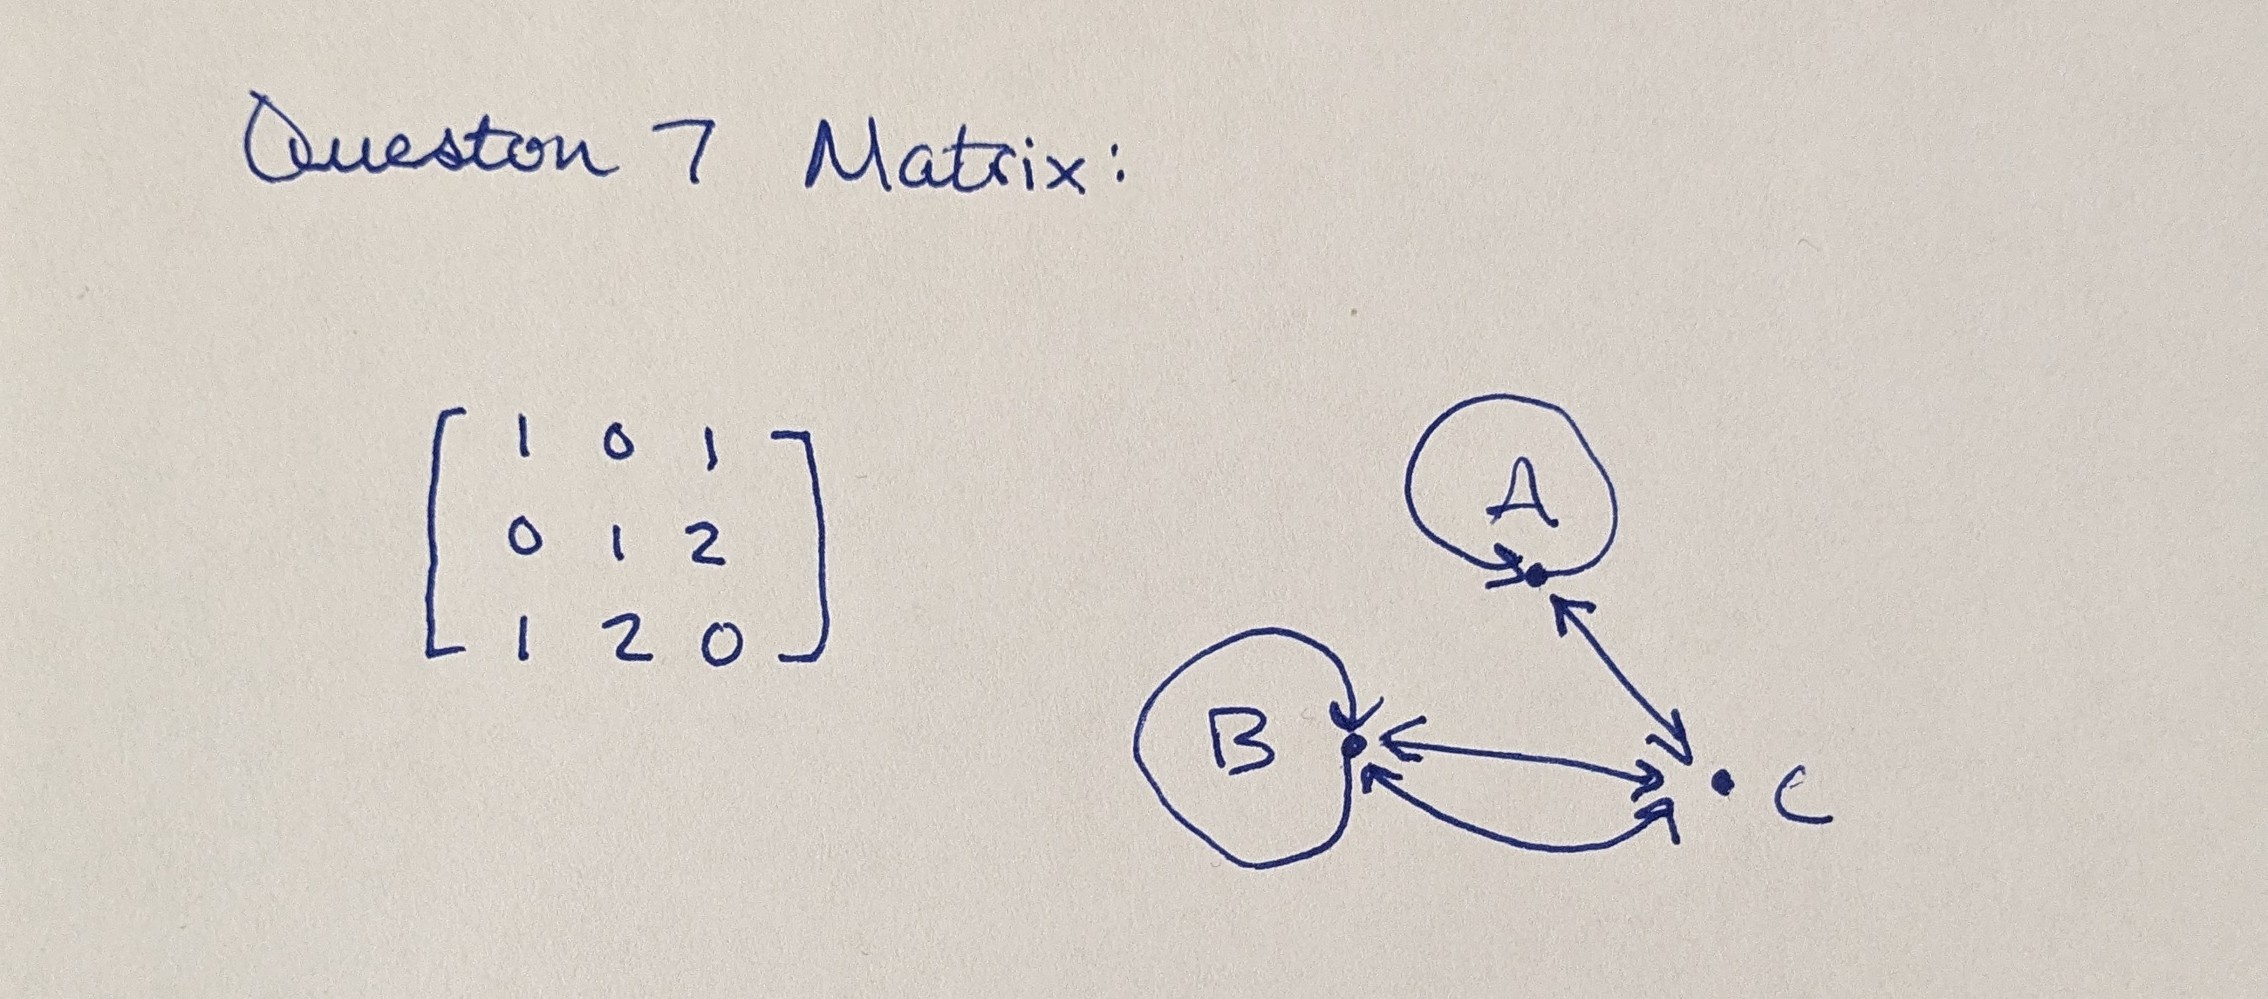
\includegraphics[width=6cm]{./Question7.jpg}
    \end{center}
  \end{problem}

  \begin{problem}{Problem 8}
    The product of these two matrices is:
    \begin{equation*}
      \begin{pmatrix}
        18 & 0 & 0 \\
        1 & -1 & 0 \\
      \end{pmatrix}
    \end{equation*}
  \end{problem}

  \begin{problem}{Problem 9}
    The trees in figure 1 are graphs $b$ and $d$. Besides them looking like trees, there are no circuits in either
    of them, which follows the definition of trees.
  \end{problem}

  \begin{problem}{Problem 10}
    The number of binary trees in figure 1 is just one. Graph $d$ is the only one that is a binary tree, since 
    for every vertex, there are at most two children. Graph $b$ is not a binary tree since vertex $c$ has three
    children.
  \end{problem}

  \begin{problem}{Problem 11}
    You can create a connected graph with 9 edges and 9 vertices. This is the sketch I did:
    \begin{center}
      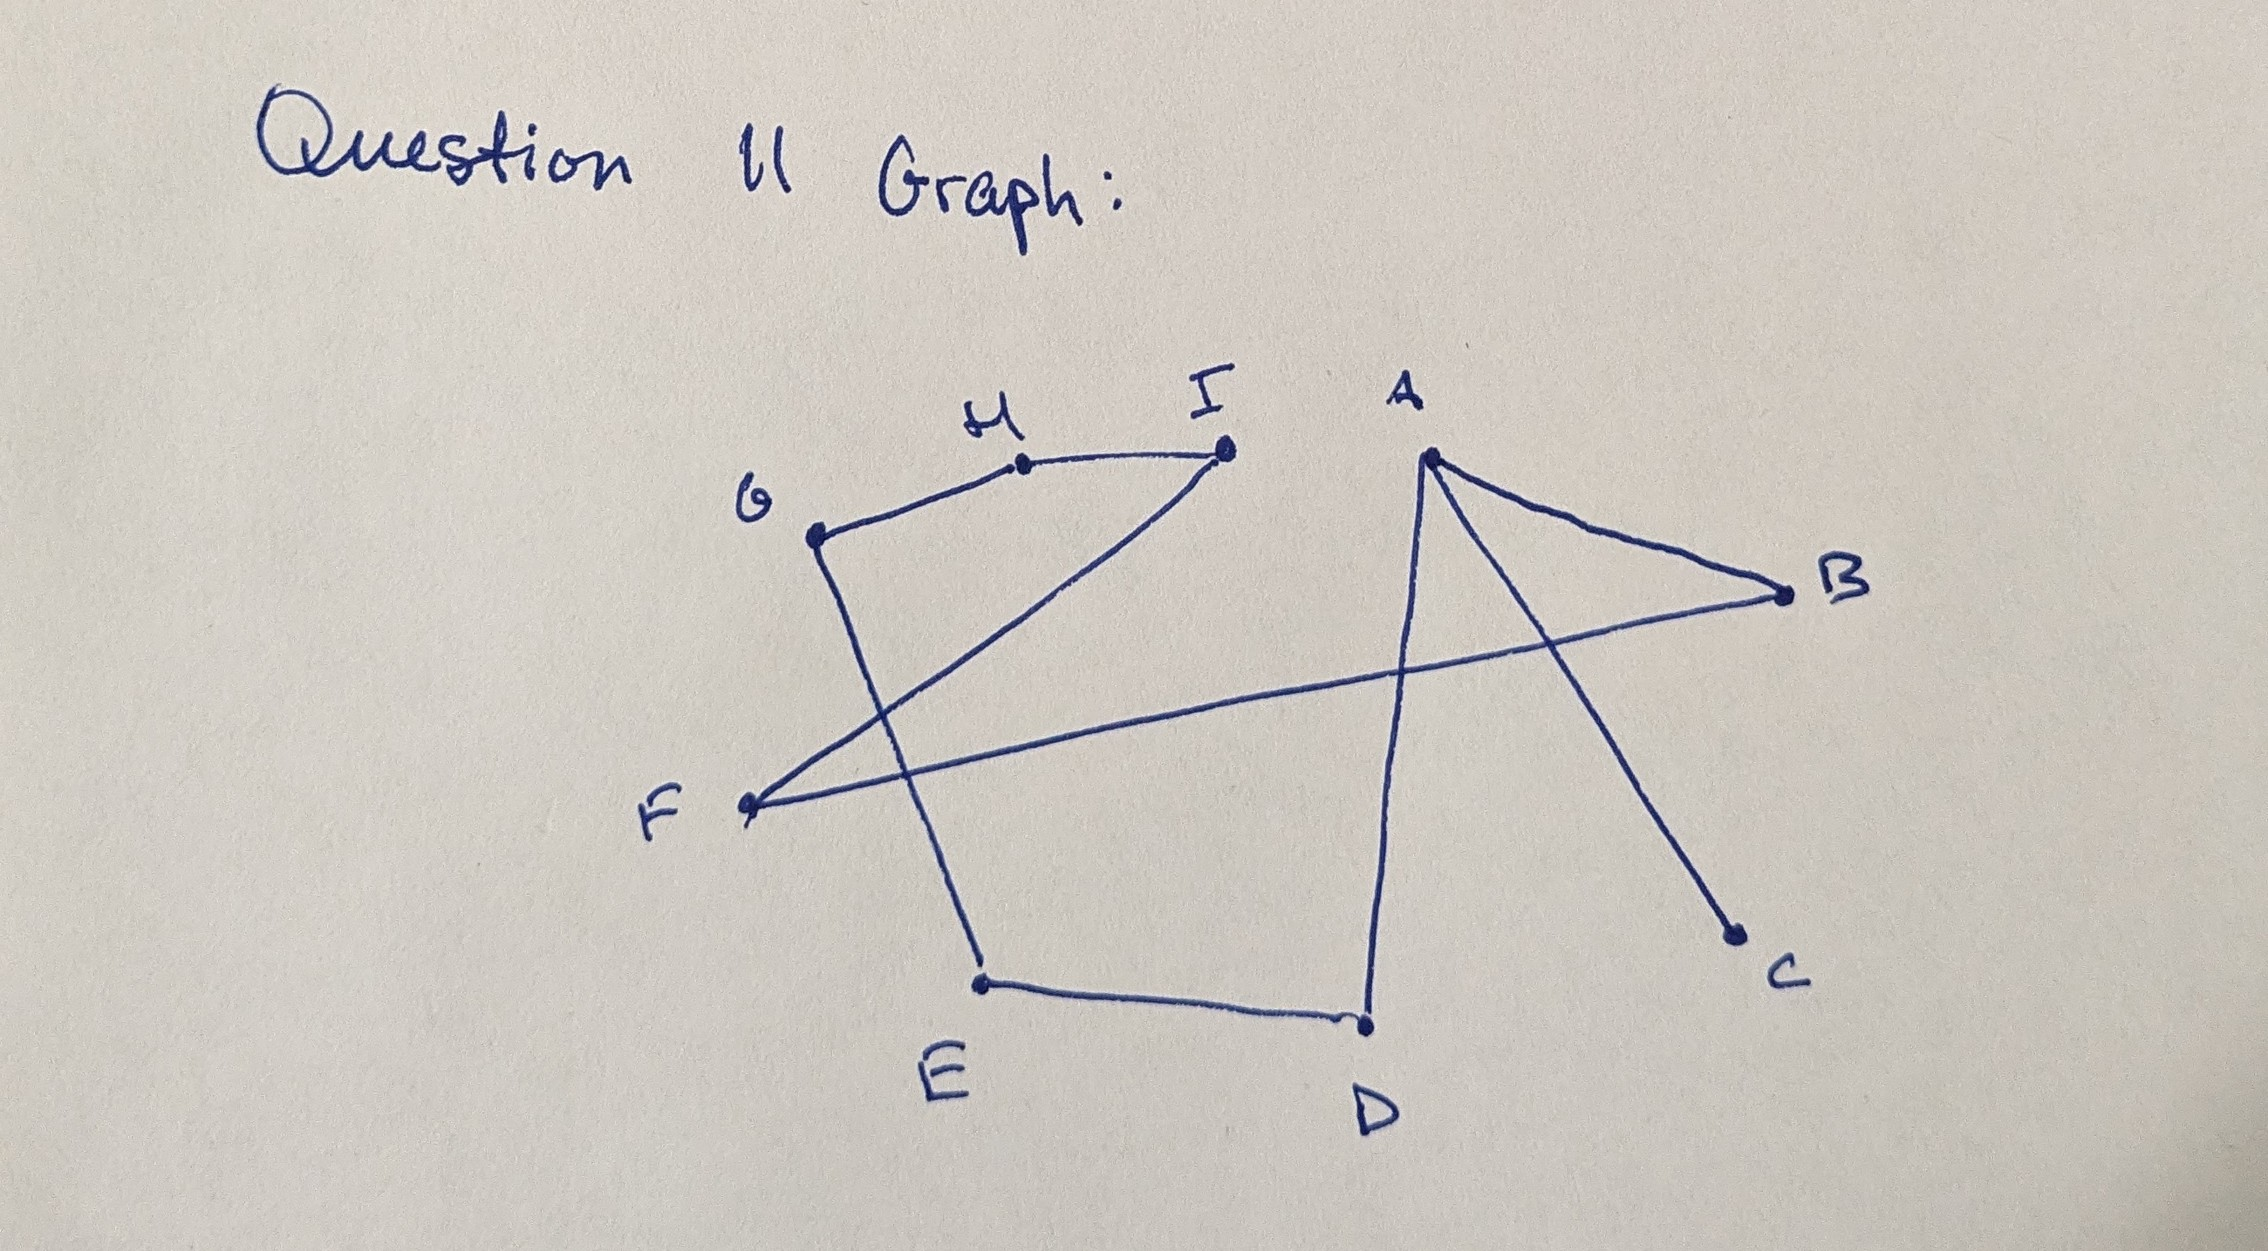
\includegraphics[width=6cm]{./Question11.jpg}
    \end{center}
  \end{problem}

  \begin{problem}{Problem 12}
    You cannot draw a tree with 9 edges and 9 vertices. Having this combination of edges and vertices would create
    at least one guaranteed circuit, which would violate the definition of a tree.
  \end{problem}

\end{document}
